\section{Implementation}
\label{sec:implementation}

The IncidentFlow ecosystem is built upon a modular architecture, separating the core language compilation from the user-facing interfaces. At the parser level, ANTLR leverages the \texttt{IncidentFlow.g4} grammar definition to translate the source text into a deeply nested Parse Tree. The sequence of language tokens navigates through the lexer to extract fundamental constructs representing triggers and phases. 

The compiler traverses this tree, checking block topologies and identifying invalid state jumps (e.g., verifying that \texttt{GOTO} expressions route securely to instanced blocks). During compilation, the engine tracks concurrent definitions encapsulated in \texttt{PARALLEL} directives, mapping them coherently to report structures rather than raw serialized logging commands. Wait behaviors map cleanly into distinct timeline expectations inside the final Markdown string. The report generation logic fundamentally hinges on a template translation pattern parsing the semantic tree sequentially, generating Markdown header blocks, and rendering an accumulative trail of \texttt{SEVERITY} adjustments.

\subsection{Command-Line Interface (CLI)}
\label{subsec:impl_cli}

The \texttt{iflow} CLI is the primary entry point for interacting with the compiler. It handles syntax validation, semantic checks, and report generation locally. The parsing sequence begins with grammar validation, followed by semantic constraint checks. A user can validate a script using \texttt{./iflow check playbooks/sample.iflow}. If valid, the CLI exits with status code 0. If it contains dangling phase references or syntax errors, it returns descriptive error logs respectively. Once verified, the \texttt{report} command compiles the playbook into a comprehensive Markdown file: \texttt{./iflow report playbooks/sample.iflow -o out.md}.

To accelerate playbook creation, the CLI includes an interactive wizard (\texttt{./iflow wizard}) that dynamically interrogates the analyst about the observed malicious behavior. By answering numerical prompts regarding attack sub-techniques (such as MITRE ATT\&CK T1566 for Phishing) and compromise scope, the CLI transpiles the parameters into a bespoke \texttt{.iflow} script and its corresponding Markdown report automatically.

\subsection{HTTP API Backend}
\label{subsec:impl_api}

To facilitate interactions from the frontend and external tools, the IncidentFlow compiler operates as a dynamic background service via the \texttt{iflow serve} command. It exposes a lightweight JSON REST API routing compilation tasks without the overhead of the CLI environment.

Crucial endpoints include:
\begin{itemize}
    \item \texttt{POST /api/compile}: Accepts arbitrary \texttt{.iflow} strings, funneling them through the parser and returning \texttt{\{ valid: true \}} on success, or structured error arrays on internal failure.
    \item \texttt{POST /api/report}: Runs the validations and appends a \texttt{report} JSON key encapsulating the final formatted Markdown string.
    \item \texttt{GET /api/playbooks}: Discovers all pre-existing \texttt{.iflow} files allocated in the server's working directory, enabling templates to be queried algorithmically.
\end{itemize}

A valid code compilation guarantees an HTTP 200, whereas malformed source texts yield an HTTP 422 Unprocessable Entity combined with explicit parser notifications. CORS support enables native decoupled frontend integration.

\subsection{Frontend Architecture and UI}
\label{subsec:impl_frontend}

The IncidentFlow frontend serves as a visual layer abstracting away the CLI restrictions, increasing accessibility for varying roles within security teams. It mirrors the CLI's utility in an intuitive, browser-based environment, relying entirely on the HTTP API backend for validation and compilation tasks.

\begin{figure}[htbp]
    \centering
    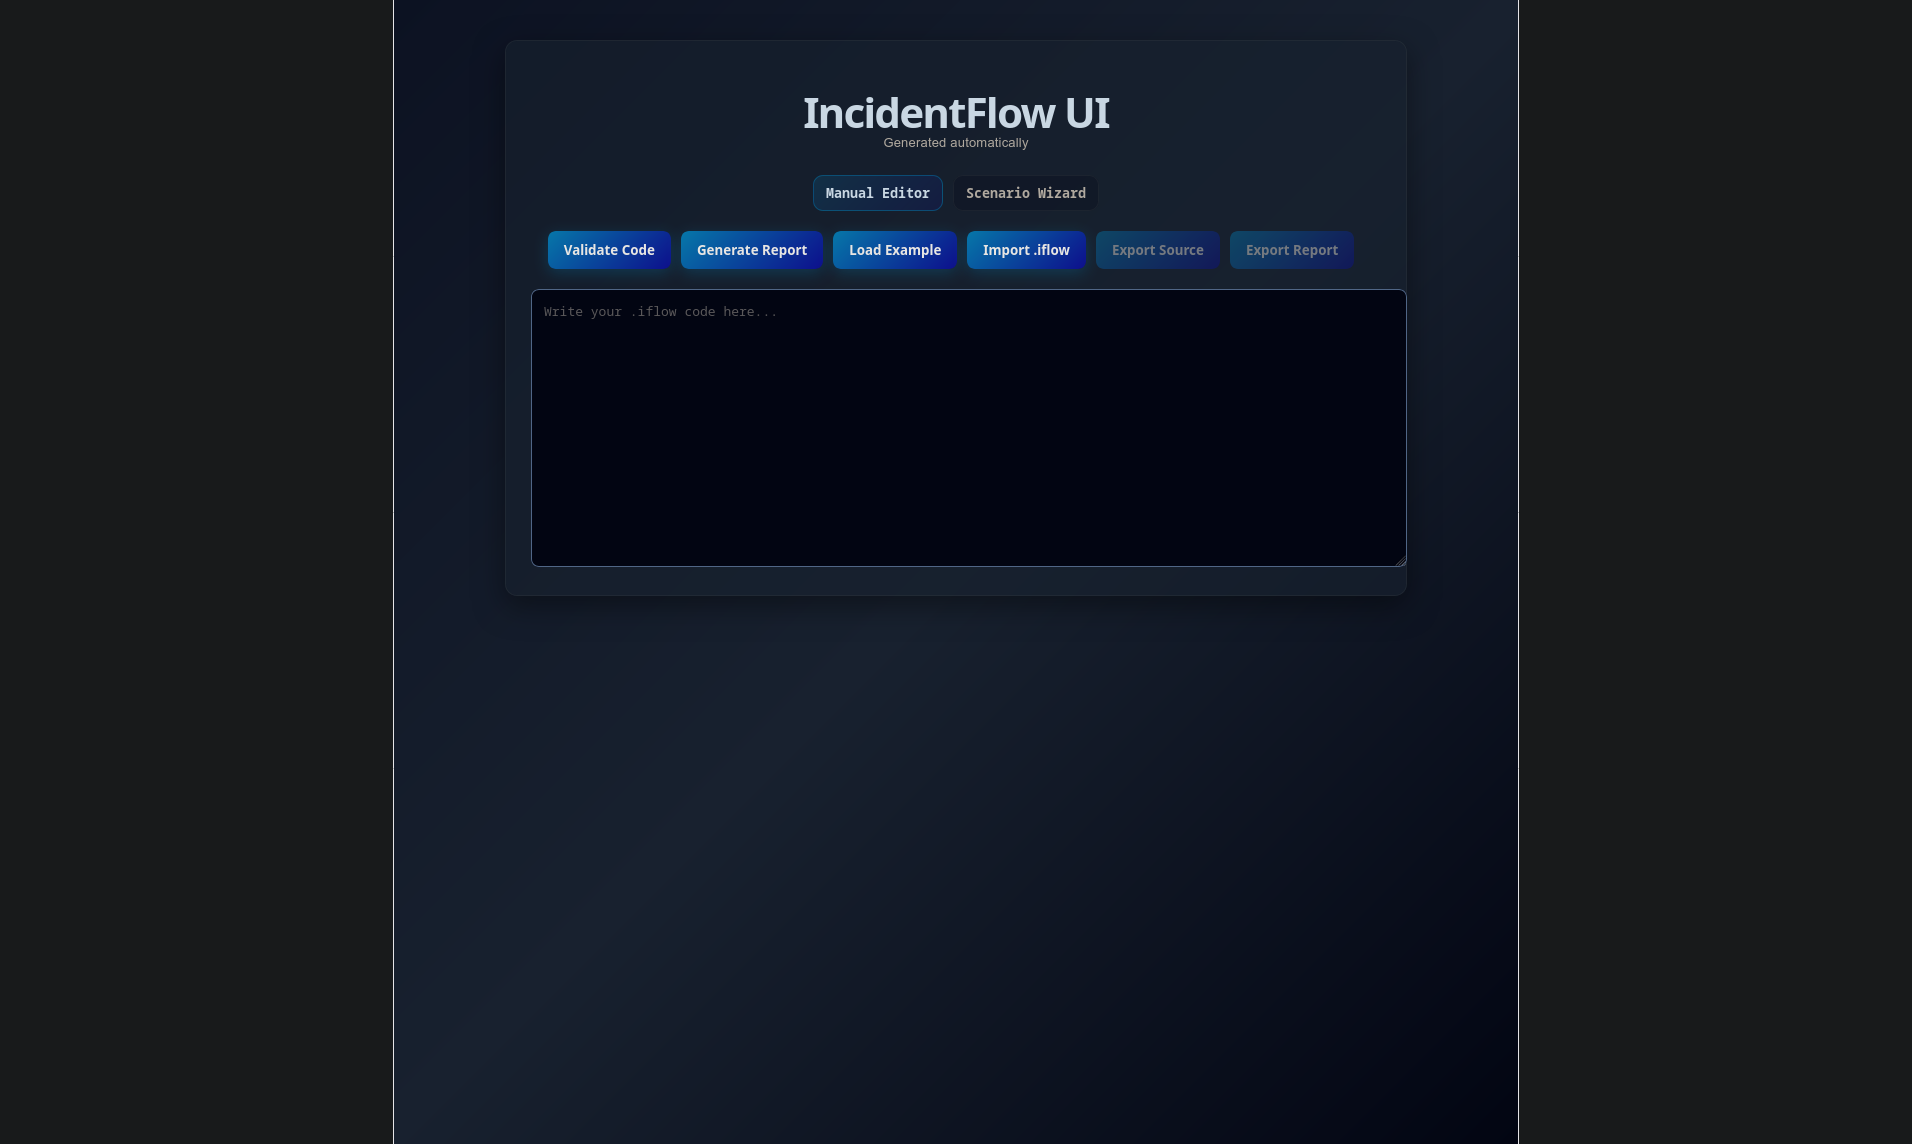
\includegraphics[width=0.8\textwidth]{images/main_page.png}
    \caption{The main editor interface of the IncidentFlow UI.}
    \label{fig:ui_main}
\end{figure}

The application provides a dual-model interaction interface: users can explicitly define scripts via the "Manual Editor" or auto-generate code via the visual "Scenario Wizard" (Figure~\ref{fig:ui_wizard}). In the Manual Editor (Figure~\ref{fig:ui_main}), text input is pushed to the API in real time.

When a user elects to generate a report from a pre-authored example, the UI loads playbooks from the backend (Figure~\ref{fig:ui_example}). If syntax or semantic faults are typed directly into the editor, the frontend catches HTTP 422 mapping errors, highlighting the exact mismatched tokens and line numbers via a red banner at the bottom of the interface (Figure~\ref{fig:ui_validate}). Finally, upon successful parsing, the frontend displays the fully templated HTML rendering of the generated Markdown (Figure~\ref{fig:ui_report_gen}), completing the visual feedback loop.

\begin{figure}[htbp]
    \centering
    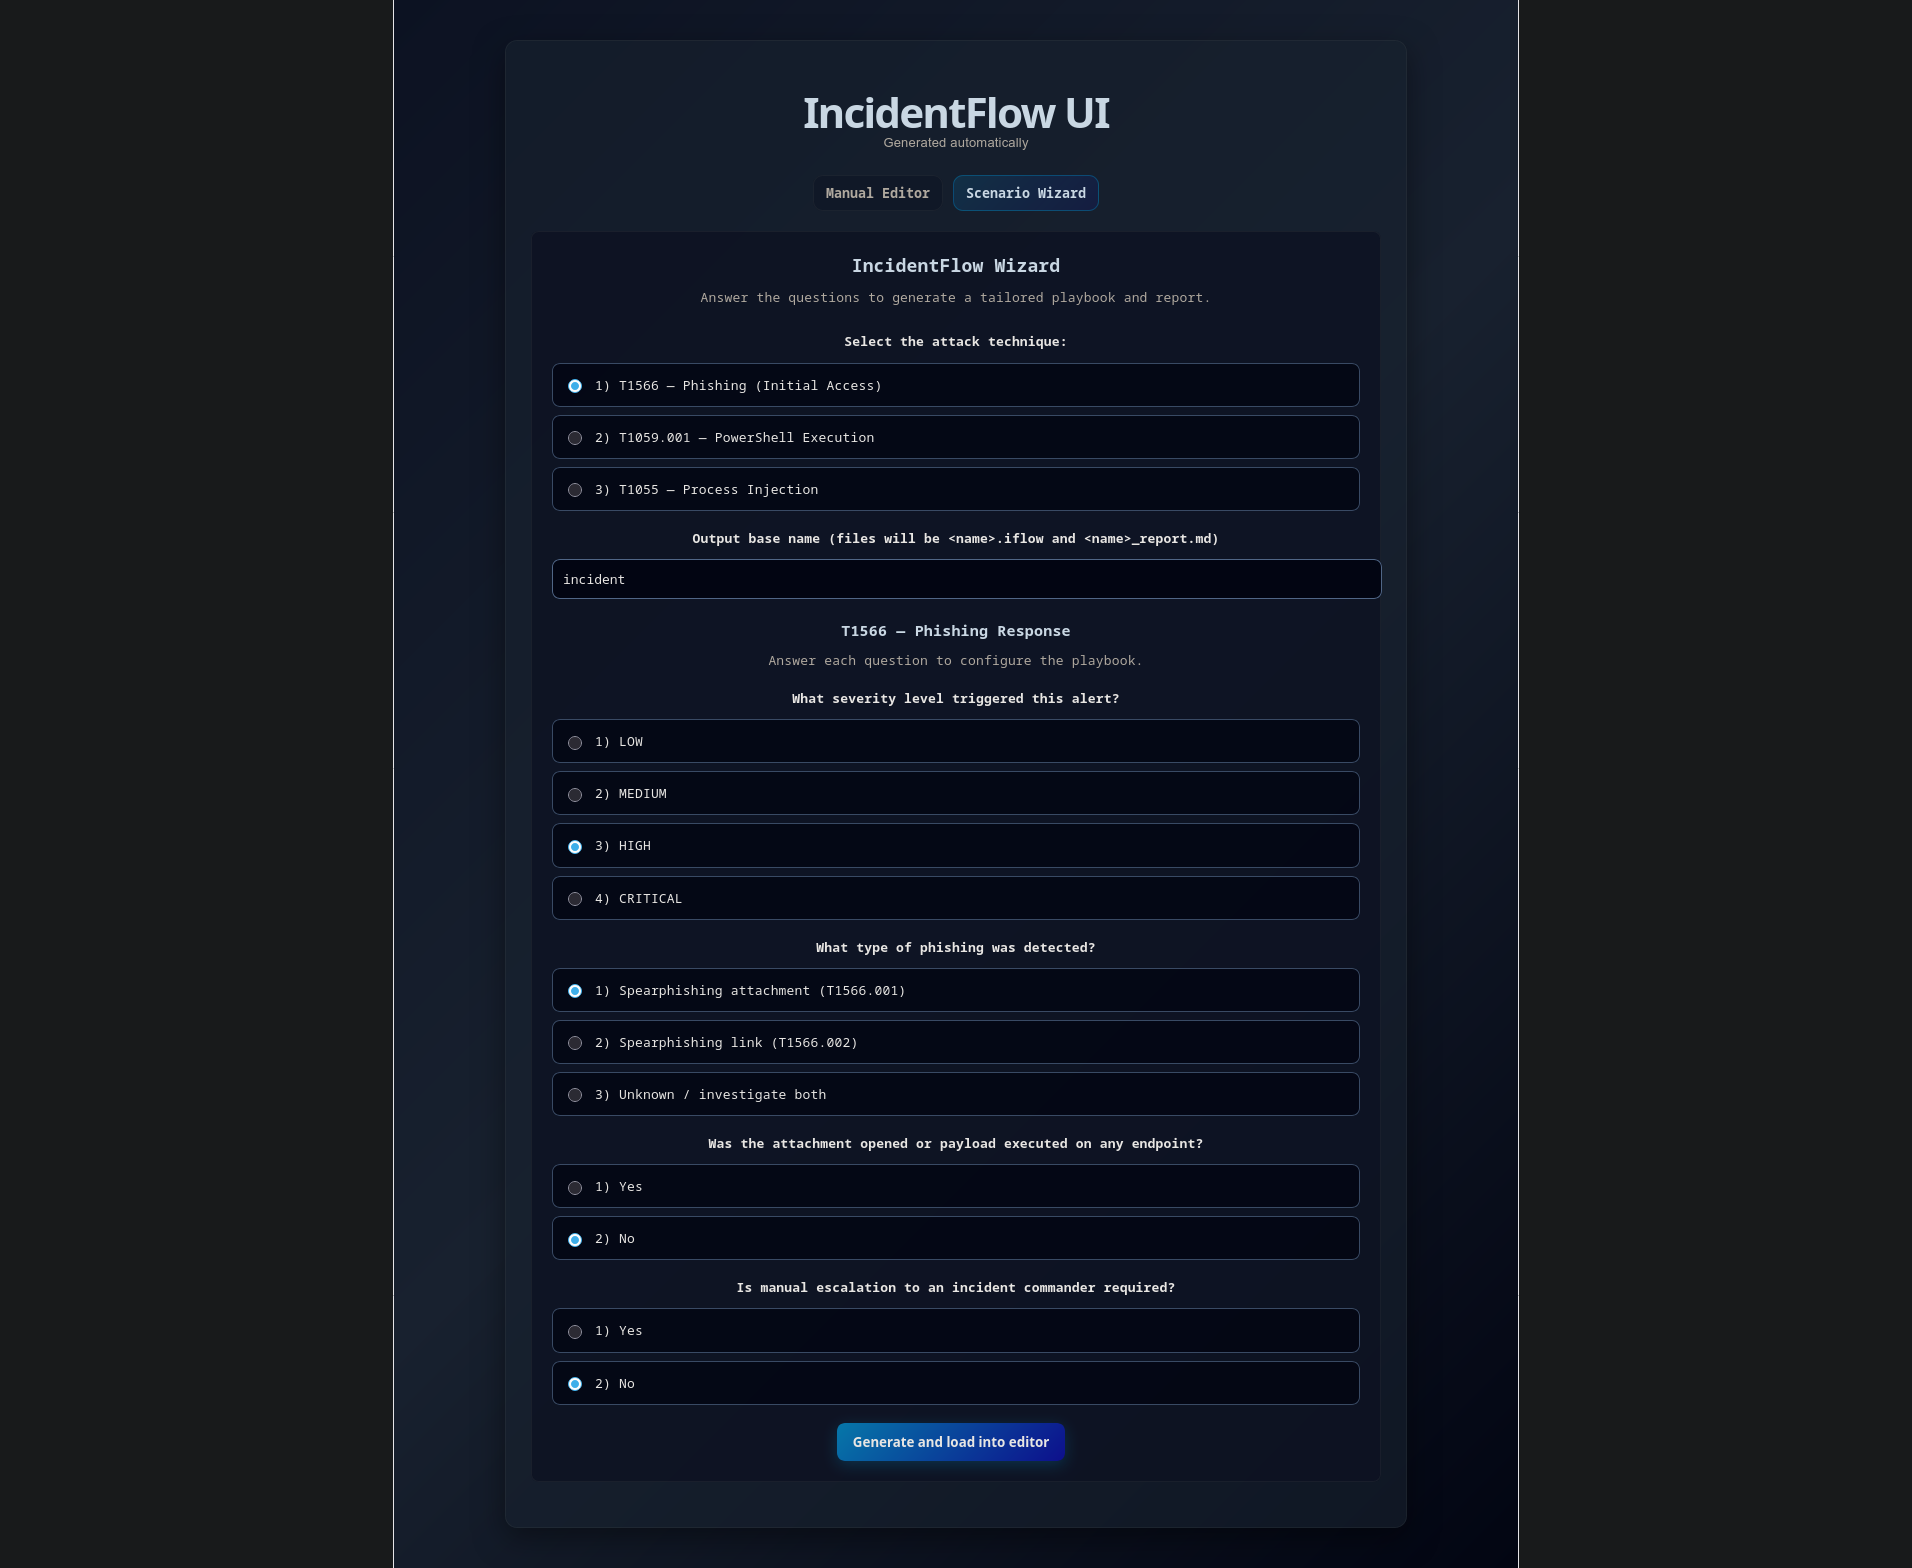
\includegraphics[width=0.8\textwidth]{images/scenario_wizard.png}
    \caption{The interactive Scenario Wizard mirroring CLI functionality in the browser.}
    \label{fig:ui_wizard}
\end{figure}

\begin{figure}[htbp]
    \centering
    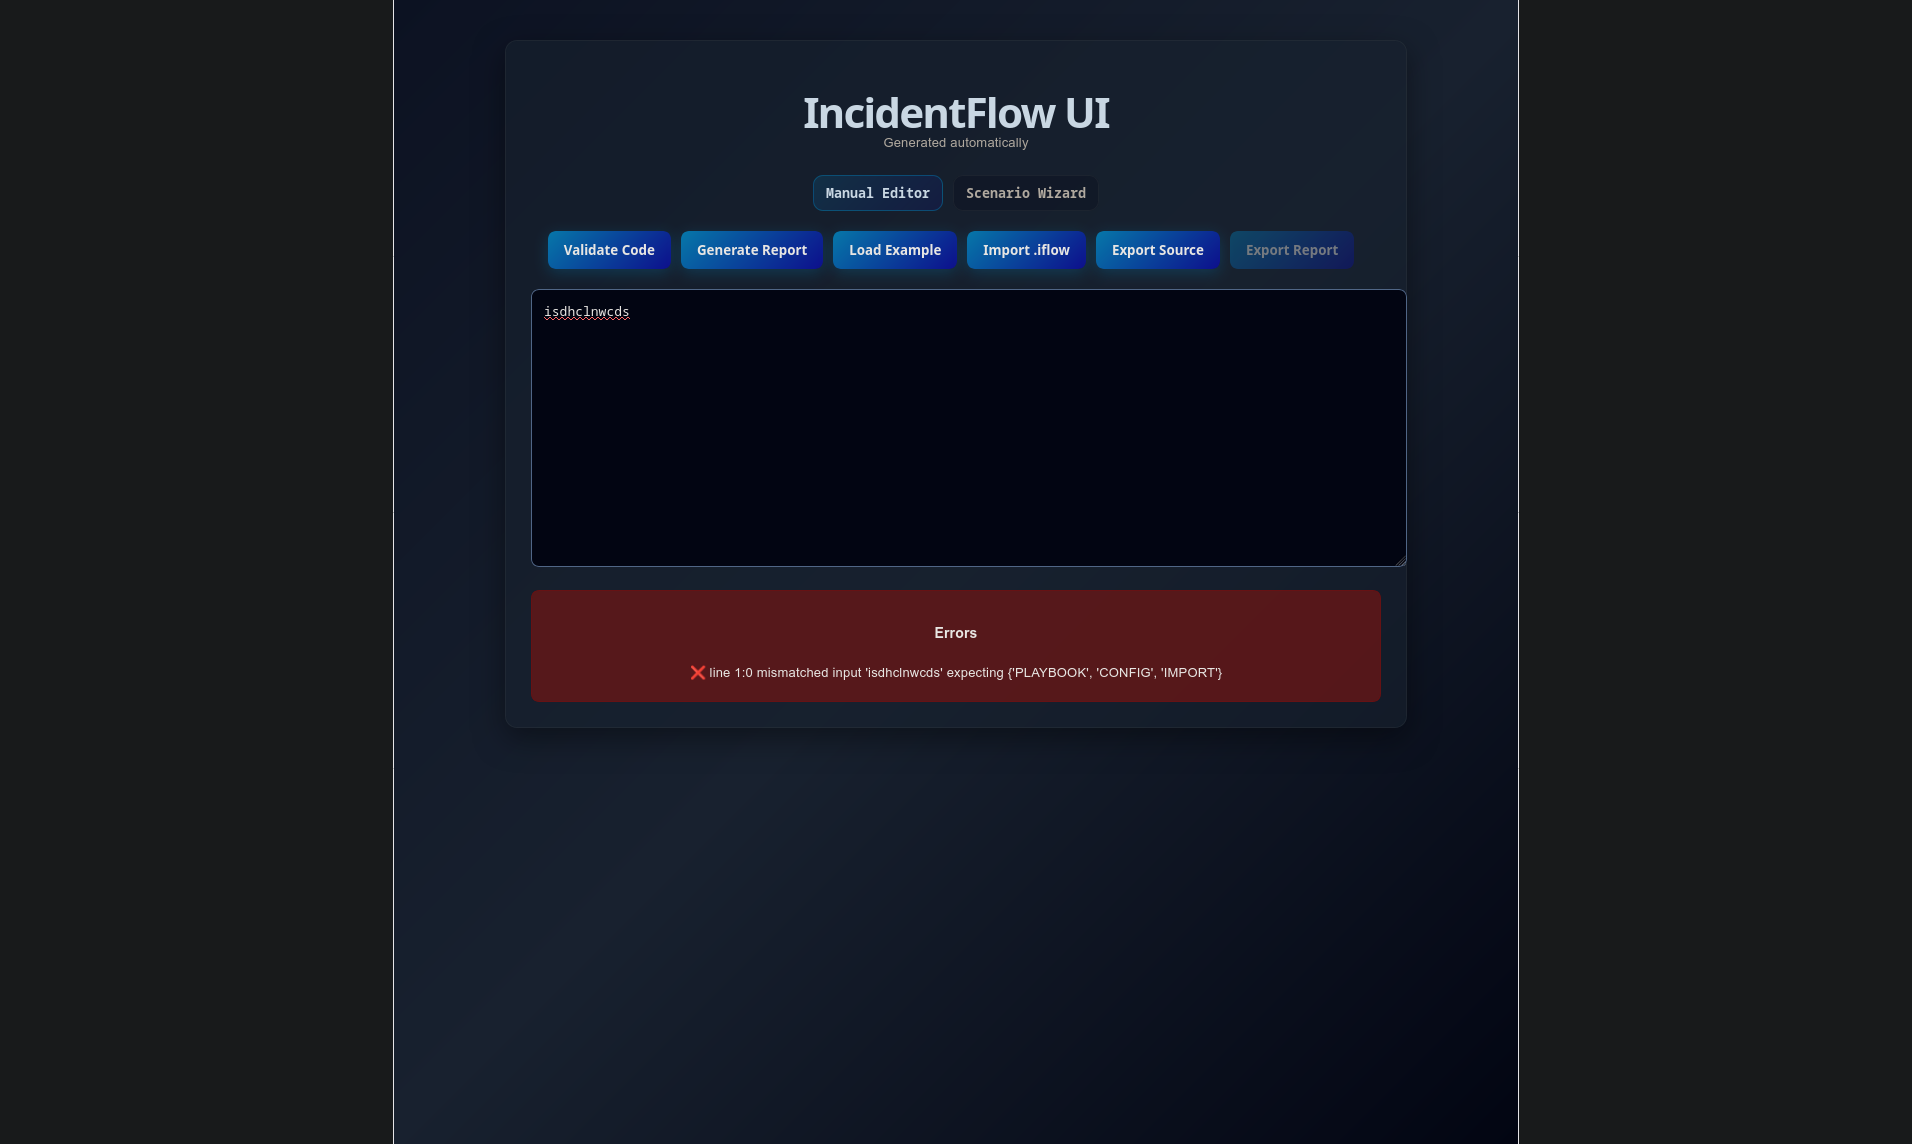
\includegraphics[width=0.7\textwidth]{images/validate_code.png}
    \caption{Syntax validation error reporting in the manual editor.}
    \label{fig:ui_validate}
\end{figure}

\begin{figure}[htbp]
    \centering
    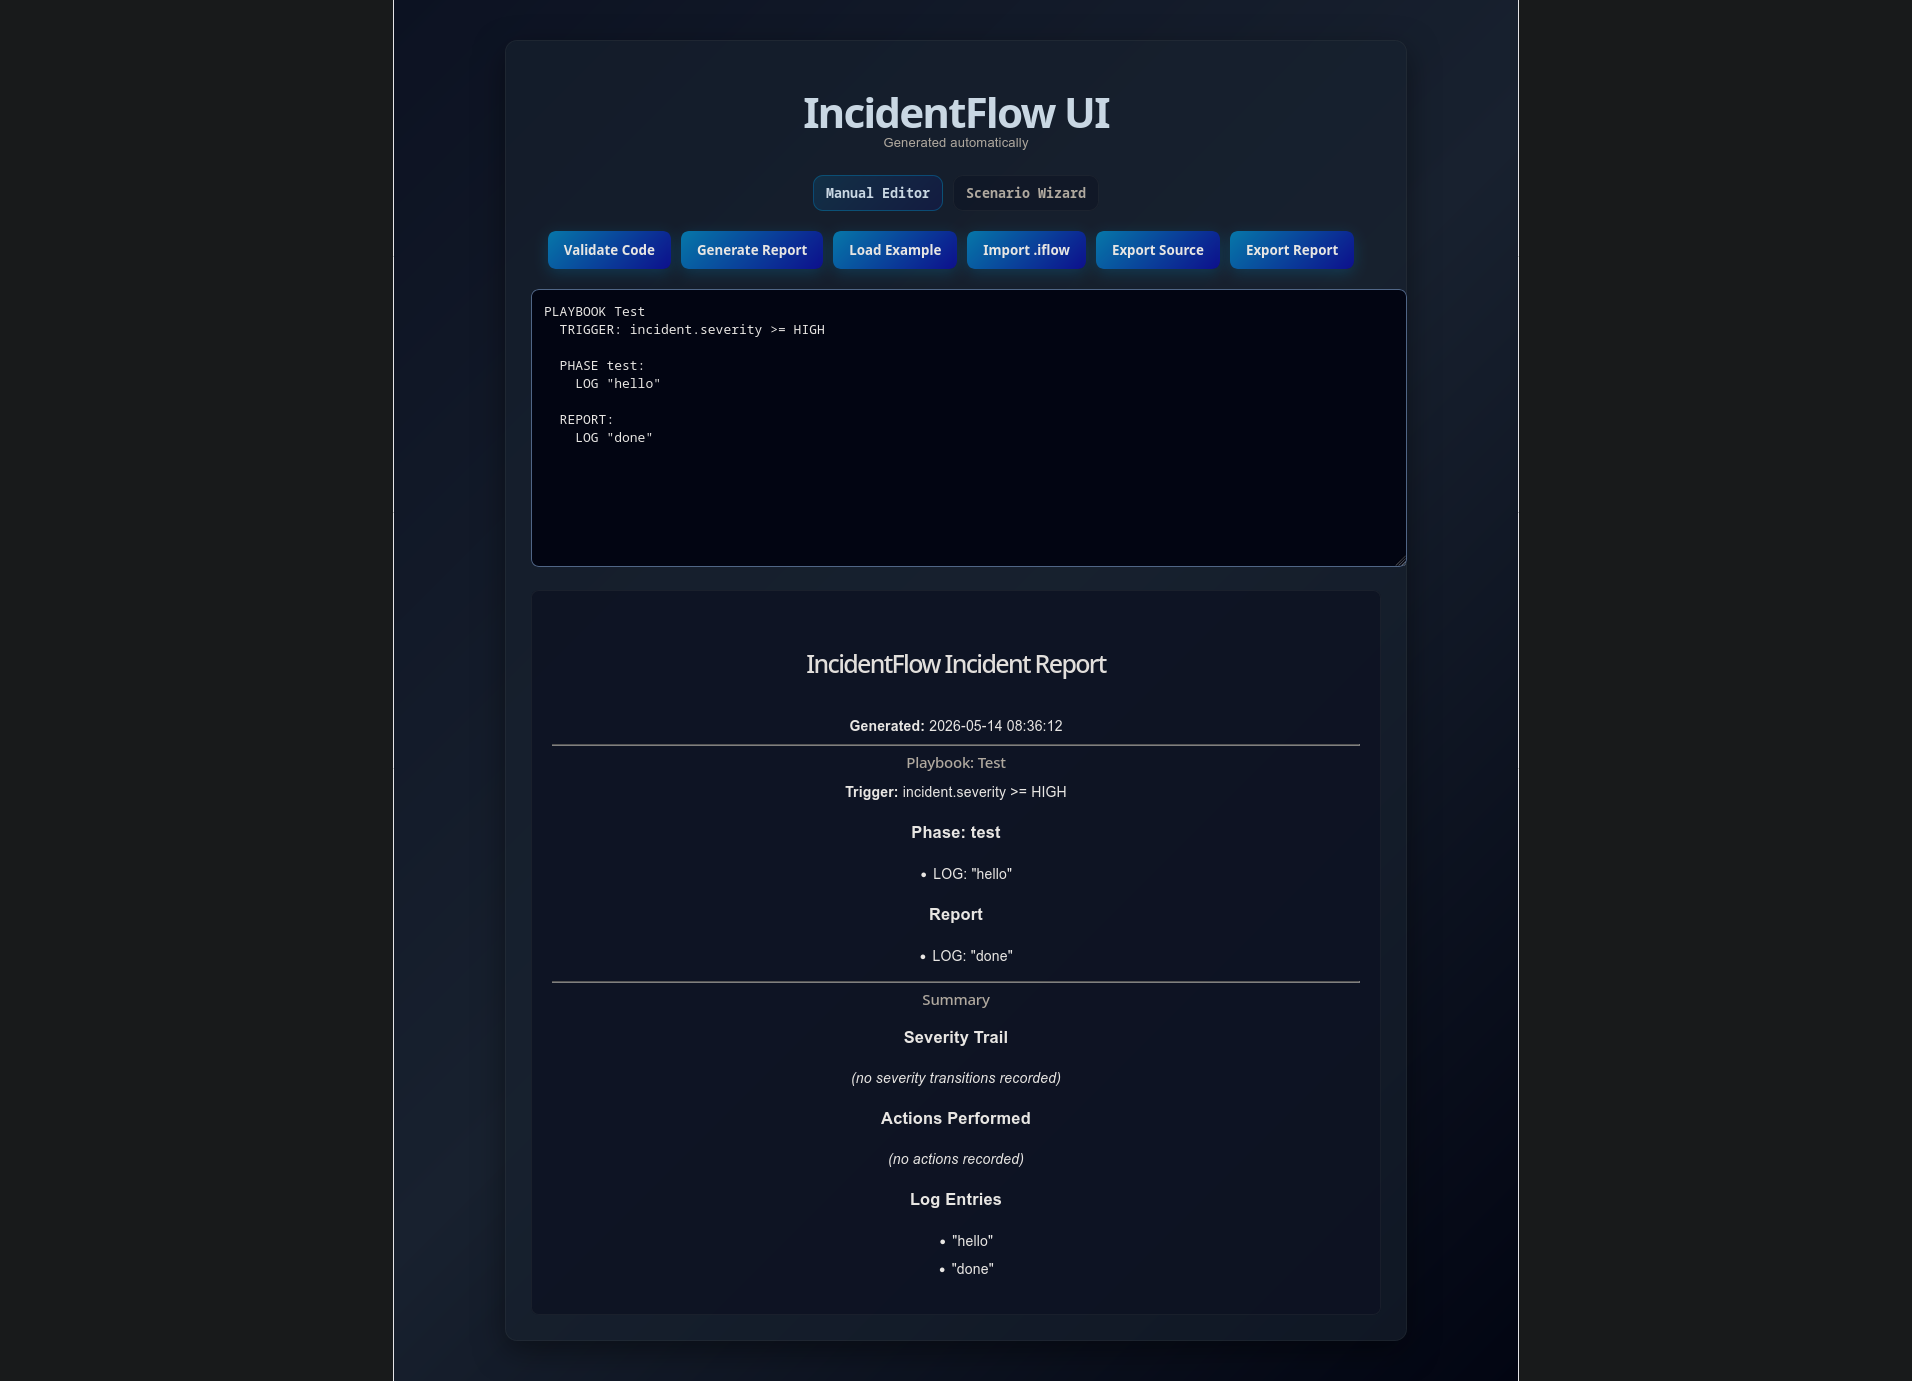
\includegraphics[width=0.8\textwidth]{images/generate_report_using_example.png}
    \caption{Loading and browsing playbook examples via the UI.}
    \label{fig:ui_example}
\end{figure}

\begin{figure}[htbp]
    \centering
    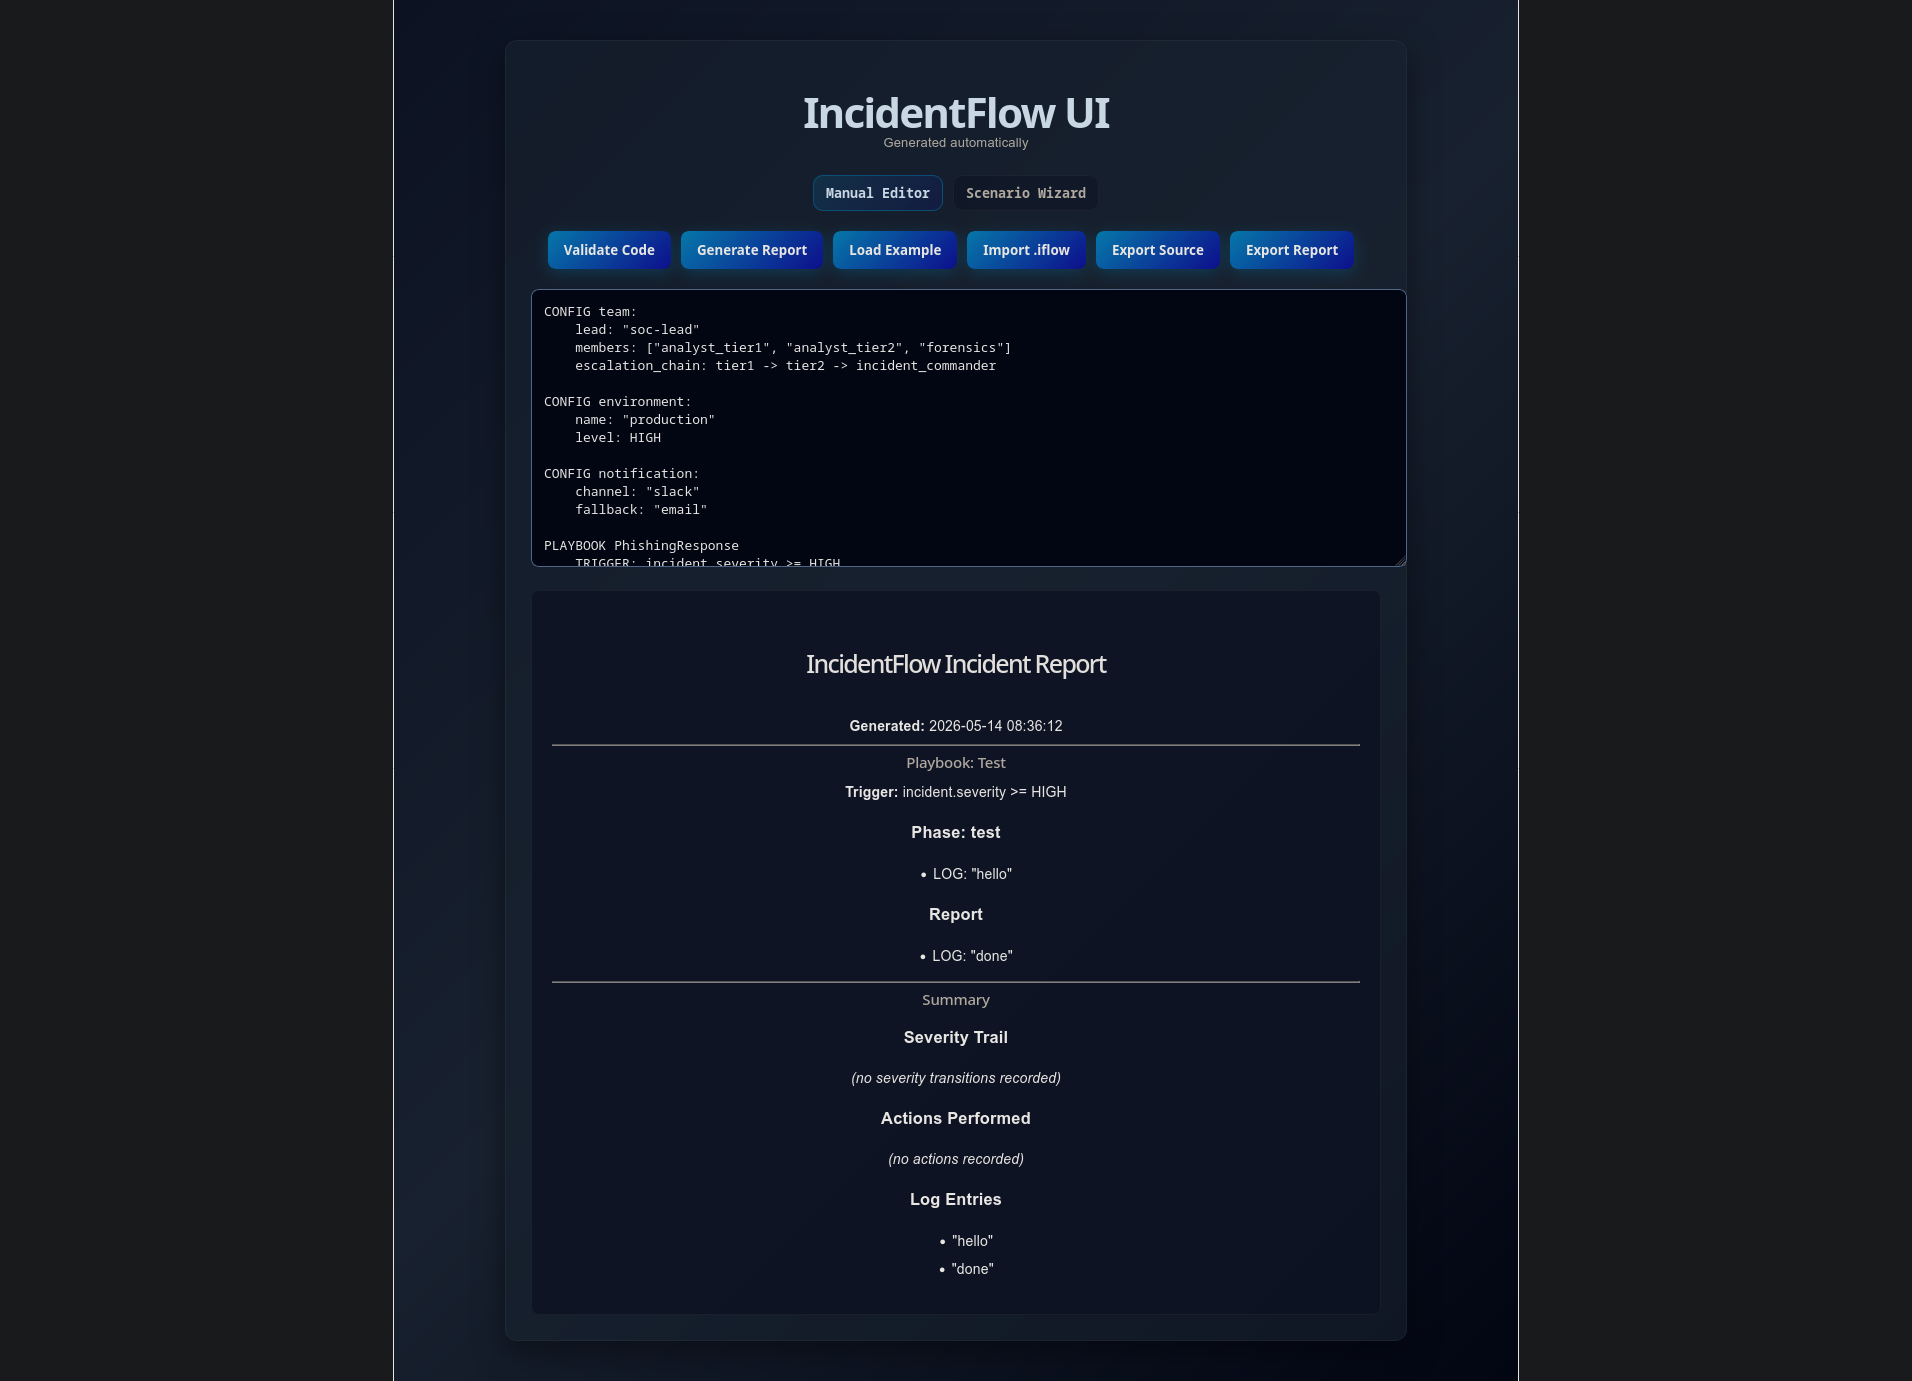
\includegraphics[width=0.8\textwidth]{images/generated_report_using_wizard.png}
    \caption{The resultant incident report rendered visually.}
    \label{fig:ui_report_gen}
\end{figure}
